\documentclass[letterpaper,11pt]{article}

\usepackage{latexsym}
\usepackage[empty]{fullpage}
\usepackage{titlesec}
\usepackage{marvosym}
\usepackage[usenames,dvipsnames]{color}
\usepackage{verbatim}
\usepackage{enumitem}
\usepackage[hidelinks]{hyperref}
\usepackage{fancyhdr}
\usepackage[english]{babel}
\usepackage{tabularx}
\usepackage{fontawesome5}
\usepackage{multicol}
\setlength{\multicolsep}{-3.0pt}
\setlength{\columnsep}{-1pt}
\input{glyphtounicode}

%new packages

\usepackage{fontenc}
\usepackage{amsmath}
\usepackage{amssymb}
\usepackage{graphicx}



%----------FONT OPTIONS----------

\pagestyle{fancy}
\fancyhf{} % clear all header and footer fields
\fancyfoot{}
\renewcommand{\headrulewidth}{0pt}
\renewcommand{\footrulewidth}{0pt}

% Adjust margins
\addtolength{\oddsidemargin}{-0.6in}
\addtolength{\evensidemargin}{-0.5in}
\addtolength{\textwidth}{1.19in}
\addtolength{\topmargin}{-.7in}
\addtolength{\textheight}{1.4in}

\urlstyle{same}

\raggedbottom
\raggedright
\setlength{\tabcolsep}{0in}

% Sections formatting
\titleformat{\section}{
  \vspace{-4pt}\scshape\raggedright\large\bfseries
}{}{0em}{}[\color{black}\titlerule \vspace{-5pt}]



% Ensure that generate pdf is machine readable/ATS parsable
\pdfgentounicode=1

%-------------------------
% Custom commands
\newcommand{\resumeItem}[1]{
  \item\small{
    {#1 \vspace{-2pt}}
  }
}

\newcommand{\classesList}[4]{
    \item\small{
        {#1 #2 #3 #4 \vspace{-2pt}}
  }
}

\newcommand{\resumeSubheading}[4]{
  \vspace{-2pt}\item
    \begin{tabular*}{1.0\textwidth}[t]{l@{\extracolsep{\fill}}r}
      \textbf{#1} & \textbf{\small #2} \\
      \textit{\small#3} & \textit{\small #4} \\
    \end{tabular*}\vspace{-7pt}
}

\newcommand{\resumeSubSubheading}[2]{
    \item
    \begin{tabular*}{0.97\textwidth}{l@{\extracolsep{\fill}}r}
      \textit{\small#1} & \textit{\small #2} \\
    \end{tabular*}\vspace{-7pt}
}

\newcommand{\resumeProjectHeading}[2]{
    \item
    \begin{tabular*}{1.001\textwidth}{l@{\extracolsep{\fill}}r}
      \small#1 & \textbf{\small #2}\\
    \end{tabular*}\vspace{-7pt}
}


\newcommand{\resumeSubItem}[1]{\resumeItem{#1}\vspace{-4pt}}

\renewcommand\labelitemi{$\vcenter{\hbox{\tiny$\bullet$}}$}
\renewcommand\labelitemii{$\vcenter{\hbox{\tiny$\bullet$}}$}

\newcommand{\resumeSubHeadingListStart}{\begin{itemize}[leftmargin=0.0in, label={}]}
\newcommand{\resumeSubHeadingListEnd}{\end{itemize}}
\newcommand{\resumeItemListStart}{\begin{itemize}}
\newcommand{\resumeItemListEnd}{\end{itemize}\vspace{-5pt}}


\begin{document}
\fontfamily{cmr}\selectfont
\begin{center}
\parbox{3.0cm}{%
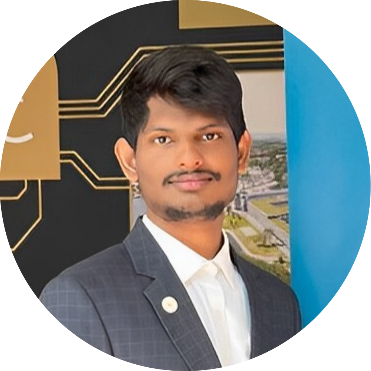
\includegraphics[width=2.7cm,clip]{images/resume_pic_m.png}}
\parbox{\dimexpr\linewidth-3.8cm\relax}{
\vspace{-20pt}
\begin{tabularx}{\linewidth}{L r} \\
    {\Huge \scshape  Venkata Sai Yakkshit Reddy Asodi}~ \href{https://www.cedzlabs.com/yakkshit}{\vspace{1pt}}\\
      Berlin, Germany. \\ \vspace{1pt}
     \small \raisebox{-0.1\height}\faPhone\ +91 8179936156 ~ \href{mailto:saiyakkshit2001@gmail.com}{\raisebox{-0.2\height}\faEnvelope\  {saiyakkshit2001@gmail.com}} ~ 
    \href{https://linkedin.com/in/yakkshit/}{\raisebox{-0.2\height}\faLinkedin\ {yakkshit}}  ~
    \href{https://yakkshit.com/}{\raisebox{-0.2\height}\faGlobe\ {yakkshit.com}}  ~
    \href{https://github.com/yakkshit}{\raisebox{-0.2\height}\faGithub{ yakkshit}}
    \vspace{-8pt}
\end{tabularx}
}
\end{center}

\vspace{-23pt}

\section{Summary}
Results-driven Software Development Engineer specializing in 5G wireless technology, embedded systems, and telecommunications. Adept in designing and maintaining high availability software for 5G base stations with expertise in C++, Python, and Linux environments. Proven ability to implement Layer 3 protocols, Agile methodologies, and software quality assurance. Seeking to contribute to innovative 5G development projects.

\section{Technical Skills}
\begin{itemize}[leftmargin=0.15in, label={}]
\small{\item{
\textbf{Languages - }{C++14, Python, Bash.} \\
\textbf{Frameworks - }{Linux, gtest, gmock.} \\
\textbf{Tools - }{Git, Gerrit, CI/CD pipelines.} \\
\textbf{Testing - }{TDD, Unit Testing, Component Testing.} \\
\textbf{Protocols - }{5G NR, LTE, O-RAN, vRAN.} \\
}}
\end{itemize}
\vspace{-10pt}

\section{Experience}
\resumeSubHeadingListStart

\resumeSubheading
{Circleup AG \faBuilding}{January 2024 -- July 2024}
  {Lead Full Stack Engineer}{Zurich, Switzerland}\\
\vspace{10pt}
\textbf{Responsibilities:}
\resumeItemListStart
\resumeItem{Developed responsive web applications using React and Django, integrating APIs with AI-driven services.}
\resumeItem{Led the UI/UX design and optimized application performance for scalability in Agile sprints.}
\resumeItemListEnd
\vspace{-3pt}
\textbf{Environment:}\emph{React, Django, AI APIs, RESTful APIs.}

\resumeSubheading
{CEDZLABS  \faBuilding}{December 2022 -- January 2024}
  {SW Engineer}{India}\\
\vspace{10pt}
\textbf{Responsibilities:}
\resumeItemListStart
\resumeItem{Designed and implemented Layer 3 control plane software for Nokia 5G base stations in a Scrum environment.}
\resumeItem{Developed and maintained high-availability software using C++ and Python, with a focus on 5G NR protocols and resource management.}
\resumeItem{Contributed to continuous integration, automated testing, and defect resolution.}
\resumeItemListEnd
\vspace{-3pt}
\textbf{Environment:}\emph{C++14, Python, Bash, Linux, 5G NR, LTE, Git, Gerrit, gtest, Agile methodologies.}

\resumeSubHeadingListEnd

\section{Projects}
\resumeSubHeadingListStart
\resumeProjectHeading
{\textbf{AI Resume Tuner} $|$ \emph{Azure Cloud, Next.js, RAG, LLMs}}{August 2023}\\
\vspace{5pt}
\resumeItemListStart
\resumeItem{Developed an AI-powered resume tuner using Retrieval Augmented Generation (RAG) and multimodal LLMs. Integrated backend APIs with a Next.js frontend, deployed on Azure Cloud.}
\resumeItemListEnd
\vspace{-5pt}

\resumeProjectHeading
{\textbf{5G Network Simulator} $|$ \emph{C++, Python, 5G Protocols}}{June 2022}\\
\vspace{5pt}
\resumeItemListStart
\resumeItem{Built a 5G network simulator to test Layer 3 protocol interactions and resource management in a gNB. Designed with C++ for protocol handling and Python for result analysis.}
\resumeItemListEnd
\vspace{-5pt}

\section{Achievements}
\resumeItemListStart
\resumeItem{Developed and optimized Layer 3 protocol handling for Nokia 5G base stations, improving software performance by 15\%.}
\resumeItem{Completed course on telecommunications projects, focused on 5G and LTE technologies by cisco.}
\resumeItemListEnd

\section*{Languages}
\begin{itemize}
  \item Telugu - Native $|$ English - Fluent $|$ German - Elementary.
\end{itemize}

\end{document}